\section{Implementazione}
Il seguente capitolo motiva e dettaglia le scelte implementative ritenute rilevanti per una corretta comprensione del progetto.


\subsection{Utilizzo paradigma funzionale}
Sin dalle prime fasi di progettazione il team ha intrapreso la scelta di utilizzare il più possibile il paradigma funzionale, cercando di non ricorrere alle usuali abitudini di programmazione object-oriented. Per fare ciò sono state utilizzate diverse metodologie: 
\begin{itemize}
    \item inutilizzo dei side effect, creando ad ogni modifica un nuovo ogetto immutabile.
    \item utilizzo di funzioni ricorsive.
    \item utilizzo di funzioni higher-order che permettono una facile ed immediata realizzazione del parttern Strategy, consentono una maggiore riutilizzabilità del codice. In questo modo è possibile passare alle funzioni strategie esterne, non necessitando così di modificare il codice.
\end{itemize}

Il Controller e il Model dell'applicazione sono state realizzate con un approccio puramente funzionale, mentre la View adotta un approccio funzionale attraverso la libreria cats.effect.IO ove possibile.


Prof: "Ricordatevi che la lettura della relazione fino a: (i) i requirement, deve essere sufficiente per uno sviluppatore per giungere ad un sistema che fa quello che fa il vostro; (ii) al design, deve essere sufficiente per uno sviluppatore per giungere ad un sistema che in più è organizzato come il vostro; (iii) alla implementazione, è essenzialmente equivalente al vostro."
\subsubsection{View}
Bisogna parlare della View, in particolare dell'approccio funzionale utilizzato.

\subsubsection{Creazione di un nuovo world ad ogni iterazione}


\subsubsection{Monadi}


\subsubsection{World e Stream}
Il World è stato modellato come un contenitore immutabile delle proprietà della simulazione e delle entità che vi partecipano. Al fine di memorizzare i dati necessari ai fini di analisi, esso è definito in termini di se stesso: la worldHistory è uno stream costituito dalle istanze di World riferite alle iterazioni precedenti. La lazy evaluation degli stream permette di non appesantire la computazione del simulationLoop con un carico di lavoro altrimenti insostenibile: impiegare una collezione non lazy come una lista avrebbe comportato la creazione di una moltitudine di strutture dati intermedie di grandissime dimensioni. 

\begin{figure}[h!]
\centering
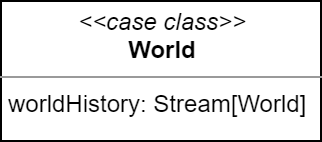
\includegraphics[scale=0.30]{img/WorldDetail.png}
\caption{Dettaglio di worldHistory come Stream per la memorizzazione delle informazioni sugli World alle iterazioni passate necessarie alla elaborazione statistica finale}
\label{fig:worldDetail}
\end{figure}

Grazie agli stream, la valutazione della grande quantità di dati accumulata avviene solo alla conclusione della simulazione e al momento del processamento dei dati a fini statistici, non interferendo così con l’andamento della simulazione.

\subsubsection{Currying e partial application}
Per incentivare il riuso, applicare il principio DRY, agevolarne l’eventuale futuro utilizzo come parametro higher order e gestire meglio l’alto numero di parametri, la funzione sinusoidal è stata implementata come funzione curried e le sue più comuni configurazioni (utilizzate più volte nel codice) sono state tramutate in partially-applied function (zeroPhasedinusoidal, zeroPhasedZeroYTranslatedSinusoidal etc). È stato utilizzato il currying anche nel codice di visualizzazione dei parametri (indicatorsUpdated di SwingView) per evitare ripetizioni di codice ed accomunare invocazioni multiple sotto la stessa signature

\subsubsection{Memoizing}



\subsection{Utilizzo della programmazione logica}
Parlo del movimento

\subsection{Test}
Prof: "Cercate di dare una idea di quanto pensate che i vostri test automatizzati coprano il codice e dove: è importante per stimare il potenziale impatto di una modifica al software." 
Io faccio un discorso generale, se c'è un aspetto particolare nei vostri test scrivetelo pure.



\subsection{Suddivisione del lavoro}
Mia introduzione iniziale

\subsubsection{Persona qualsiasi}
Ognugno deve dire cosa ha fatto, la sezione di progetto riconducibile a lui (es: per Vaio l'IA e il disegno delle statistiche finali) e se ha collaborato con qualcuno.

\subsubsection{Rei Beshiri}
Il mio ruolo nel progetto dal punto di vista implementativo riguarda principalmente lo sviluppo del model e delle sue diverse componenti in collaborazione con i membri del team, in particolare delle entità \textit{blob} del loro comportamento e reazione all'ambiente circostante e alle intersezioni tra le varie entità in gioco e degli effetti delle stesse così come della loro bounding box.

I test sviluppati riguardano le classi \code{BlobTest}, \code{DegradationTest}, \code{IntersectionTest}.

\subsubsection{Andrea Betti}
Ho contribuito insieme a Rei Beshiri all'implementazione dei comportamenti delle diverse entità della simulazione in \code{evo\_sim.model.EntityBehaviour} e agli effetti applicabili dalle entità \textit{Effectful} in \code{evo\_sim.model.effects.CollisionEffect}, realizzando le classi e le funzioni relative alle entità \textit{Food} e \textit{Plant} e contribuendo in misura minore ai comportamenti delle entità \textit{Blob} e all'estensione di \code{evo\_sim.model.EntityStructure}.

Ho inoltre implementato la logica di rappresentazione della simulazione utilizzando \texttt{scala-swing} all'interno della classe \code{evo\_sim.view.swing.custom.components.ShapesPanel}, utilizzata nella funzione \code{rendered} di \code{evo\_sim.view.swing.SwingView} realizzata da Alessandro Oliva.

Per quanto riguarda i test, ho realizzato \code{FoodTests} e \code{PlantTests}.

\subsubsection{Daniele Giulianini}

\subsubsection{Alessandro Oliva}
Il mio contributo nel model è consistito nello sviluppo delle entità \textit{Obstacle}, le entità con status temporanei (il cui raffinamento è però stato curato da Rei Beshiri), in particolare lo \textit{SlowBlob}.

Mi sono occupato inoltre del ciclo giorno notte della simulazione, con rispettiva influenza sui blob in termini di velocità e campo visivo tramite appositi moduli di funzioni.

Per quanto riguarda la View, ne ho seguito lo sviluppo dalla prima versione in \texttt{ScalaFX} fino all'implementazione puramente funzionale attraverso il framework \texttt{Cats}, del quale con l'importante contributo di Daniele Giulianini è stato sviluppato un intero package che permette di utilizzare componenti Swing in maniera funzionale. Sempre con Daniele Giulianini mi sono occupato dell'integrazione fra View e Core mediante il framework monadico. Parallelamente a questa versione è stata sviluppata un interfaccia a linea di comando per permettere la fruizione dell'applicazione nella sua interezza anche mentre si lavorava alla View.

I test da me sviluppati sono inclusi in \code{ObstacleTests}.
\subsubsection{Andrea Vaienti}